%% Template for EU deliverable, using the deliverable.sty style file

\documentclass[12pt,a4paper,twoside]{article}

%% common package
\usepackage[headers]{deliverable}
\usepackage{xspace}
\usepackage{verbatim}
\usepackage[usenames]{color}
\usepackage[usenames,dvipsnames]{xcolor}
\usepackage{graphicx}
\usepackage{url}
\usepackage{array}
\usepackage{multirow}
%%

%%insert here other packages needed by sections

%%

%%%%%%%%%%%%%%%%%%%%%%%%%%%%%%%%%%%%%%%%%%%%%%%%%%%%%%%%%%%%%%%%%%%%%%%%%%%%%%
%%% Titlepage
%%%%%%%%%%%%%%%%%%%%%%%%%%%%%%%%%%%%%%%%%%%%%%%%%%%%%%%%%%%%%%%%%%%%%%%%%%%%%%

% declaration of variables used in style
\deliverableDocnumber{D6.1}
\deliverableTitle{Website and repository on-line.}

\deliverableAuthor{Francesco Nori}
\deliverableResponsiblePartner{IIT}
\deliverableAffiliation{% Insert here authors affiliations
 $^1$ IIT 
}

\deliverableReviewer{Name of internal reviewer}
\deliverableCoordinator{Francesco Nori}
\deliverableActivityNumber{n} %% n=1,..,10
\deliverableActivity{RTD}
\deliverableDoctype{Deliverable} %% or Prototype
\deliverableClassification{Public} % or Consortium
\deliverableDistribution{Consortium} %
\deliverableStatus{Draft} % Draft or Final
\deliverableDeliveryDate{28/2/2014}
\deliverableFile{D6.1.pdf} % please do not use "-" in the name
\deliverableVersion{1.0}
\deliverableDate{Feb.~28, 2014}
\deliverableYear{2014}
\deliverablePages{\pageref{LastPage}}
\deliverableChangelog{v.1.0 & Feb 17, 2013 & First draft %%\\\hline
%%              v.2.0 & Feb 20, 2007 & Final version
}
\deliverableProjectStartingDate{1st March 2013}
\deliverableProjectEndDate{28th February 2017}
\deliverableProjectAcronym{CoDyCo}
\deliverableProjectTitle{Whole-Body Compliant Dynamical Contacts in Cognitive Humanoids}
 \deliverableContractNumber{600716}
 \deliverableProjectCoordinator{Istituto Italiano di Tecnologia}
 \deliverableProjectUrl{www.codyco.eu}
 \deliverableFrameworkProgramme{FP7}
 
 \deliverableWorkpackage{deliv WP6}
 \deliverableEditors{Francesco Nori}
 \deliverableContributors{Francesco Nori, Bruchi Alessandro}
 \deliverableReviewers{}
\deliverableAbstract{The present deliverables describes the major design solution which have been implemented in the CoDyCo website \url{www.codyco.eu}. The website is quite standard and realized with Joomla,  free and open-source content management framework (CMS) for publishing web content. The website is realized with a frontend (public and visible to the entire network) and a backend (access restricted to administrators). Simple editing can be achieved through the frontend but only registered users can edit a limited set of pages. Advanced editing is possible via the backend accessible only to website administrators.}
\deliverableReviewers{}
\deliverableKeywordList{CoDyCo, website, dissemination, results, consortium, list of publications.}

%%%%%%%%%%%%%%%%%%%%%%%%%%%%%%%%%%%%%%%%%%%%%%%%%%%%%%%%%%%%%%%%%%%%%%%%%%%%%%
%%% Sections
%%%%%%%%%%%%%%%%%%%%%%%%%%%%%%%%%%%%%%%%%%%%%%%%%%%%%%%%%%%%%%%%%%%%%%%%%%%%%%

%% constants
\newcommand{\botegoCaps}{BOTEGO}
\newcommand{\certhCaps}{CERTH}
\newcommand{\cybionCaps}{CYBION}
\newcommand{\nuigCaps}{NUIG}
\newcommand{\ubitechCaps}{UBITECH}

%%
%%%%%%%%%%%%%%%%%%%%%%%%%%%%%% BEGIN DOCUMENT
\begin{document}

\deliverableMaketitle

%%TODO move to style
\newcolumntype{L}[1]{>{\raggedright\let\newline\\\arraybackslash\hspace{0pt}}m{#1}}
\newcolumntype{C}[1]{>{\centering\let\newline\\\arraybackslash\hspace{0pt}}m{#1}}
\newcolumntype{R}[1]{>{\raggedleft\let\newline\\\arraybackslash\hspace{0pt}}m{#1}}

\textbf{Document Revision History}
\begin{center}
\begin{tabular}{|C{2cm}|C{3cm}|p{5cm}|C{4cm}|}
\hline
\textbf{Version}&\textbf{Date}&\textbf{Description}&\textbf{Author}\\\hline
First draft & 17/02/2014 & Website screen-shots added & Francesco Nori\\\hline
\end{tabular}
\end{center}
 
 \clearpage

\newpage
\renewcommand*\contentsname{Table of Contents}
\renewcommand*\listfigurename{Index of Figures}
\tableofcontents
\newpage
\listoffigures
\newpage

%%%%%%%%%%%%%%%%%%%%%%%% Start deliverable content here.

\section{Introduction}

This document describes the CoDyCo website \url{www.codyco.eu}. The goal of the website is to present the structure of the consortium and the results achieved within the CoDyCo project.

\section{Executive Summary}

This deliverables is organized as follows. Section \ref{sec:struct} presents the overall structure of the website focusing on the menu organization. Section \ref{sec:screen} presents and discusses some website screen-shots. Finally Section \ref{sec:tech} presents the website technical details.

\section{Website structure} \label {sec:struct}
The structure of the main website is represented in the following table.
\begin{center}
\begin{tabular}{ |p{3cm}|p{3cm}|p{3cm}| }
  \hline
  \multicolumn{3}{|c|}{CoDyCo banner} \\
  \hline
  \multicolumn{3}{|c|}{Main menu} \\
  \hline
  Links to funding agency and relevant projects. & Main page.  & Search engine, latest news menu and Twitter feed.\\
  \hline
\end{tabular}
\end{center}
The main menu has the following structure.
\begin{center}
\begin{tabular}{ |p{1.5cm}|p{1.5cm}|p{1.5cm}| p{1.5cm}|p{1.5cm}|p{1.5cm}|p{1.5cm}|p{1.5cm}|}
  \hline
  \multicolumn{8}{|c|}{Main menu} \\
  \hline
  Home & Partners & Scenarios & Results & Events & Team & Thanks & Login\\
  \hline
\end{tabular}
\end{center}
The home and scenarios section presents the main concept behind CoDyCo. The partners and team menus give a list of institutions and persons involved respectively. The main sub-menus are the results and events sub-menus. Their structure is in the following tables.
\begin{center}
\begin{tabular}[c]{ |p{1.5cm}|p{1.5cm}|}
  \hline
  \multicolumn{2}{|c|}{Results} \\
  \hline
   & Software\\
   & Videos\\
   & Papers\\
   & Pictures\\
  \hline
\end{tabular}
\hspace{3cm}
\begin{tabular}[c]{ |p{2cm}|p{4cm}|}
  \hline
  \multicolumn{2}{|c|}{Events} \\
  \hline
   \multirow{2}{*}{Workshops} & Workshop 1 \\
    & Workshop 2 \\
    & $\vdots$ \\
    & Workshop n \\
\cline{1-2}
   \multirow{2}{*}{Meetings} & Meeting 1\\
    & Meeting 2\\
    & $\vdots$ \\
    & Meeting m \\
  \hline
\end{tabular}
\end{center}

Another important component of the CoDyCo project is the software repository currently hosted by GitHub, is a web-based hosting service for software development projects that use the Git revision control system. The CoDyCo software repository is available here: \url{https://github.com/robotology/codyco}. Associated to the software repository there is another important website, which hosts the software documentation: \url{http://wiki.icub.org/codyco/dox/html/index.html}. The software documentation is created automatically out of the software source files with Doxygen, a tool for writing software reference documentation.

\section{Screen shots} \label{sec:screen}

\begin{figure}[h!]
    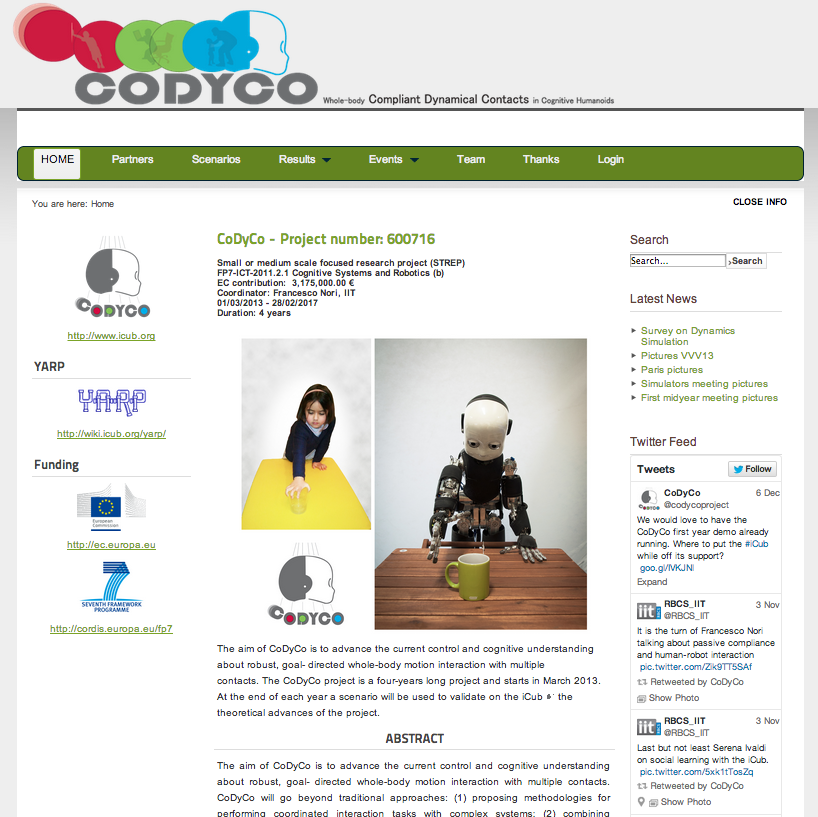
\includegraphics[width=0.45\textwidth]{images/mainWeb.png} 
    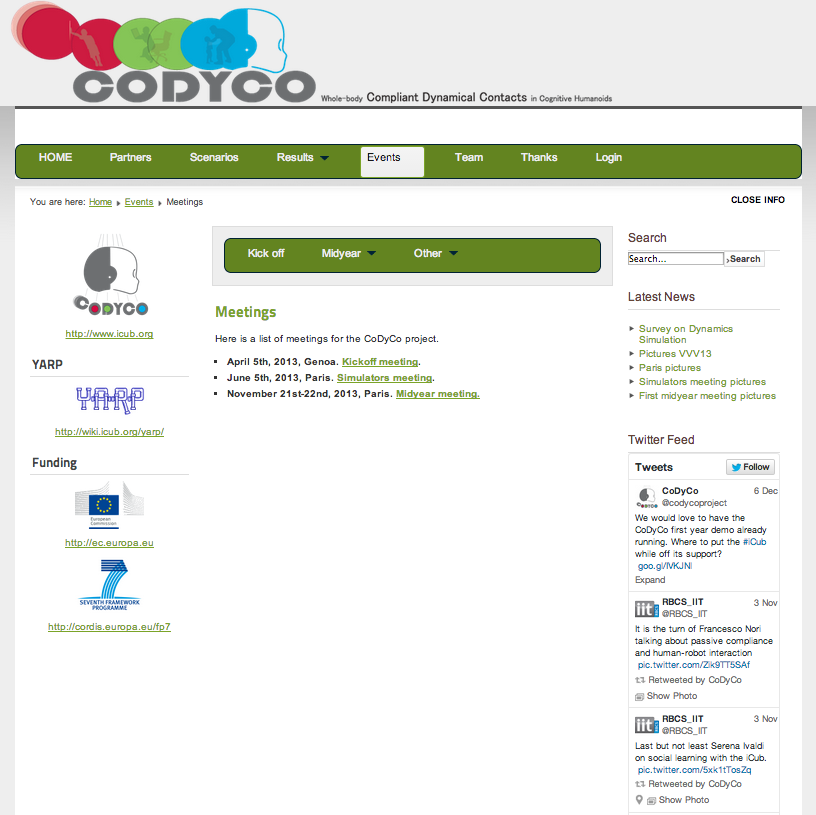
\includegraphics[width=0.45\textwidth]{images/meetingsWeb.png} \\
\vspace{0.5cm} \\
    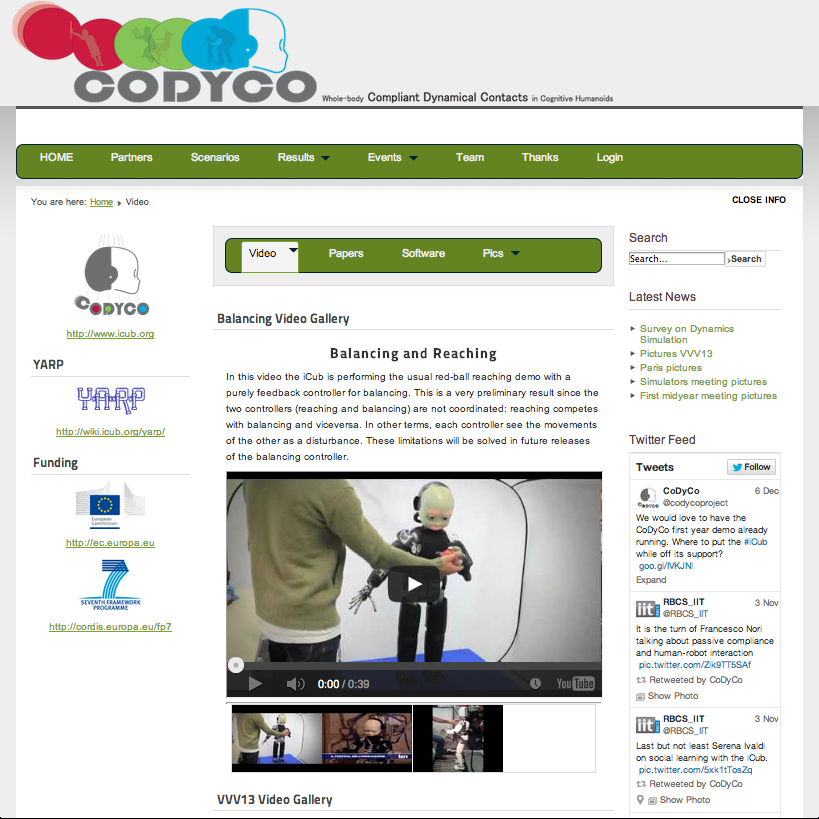
\includegraphics[width=0.45\textwidth]{images/videosWeb.png} 
    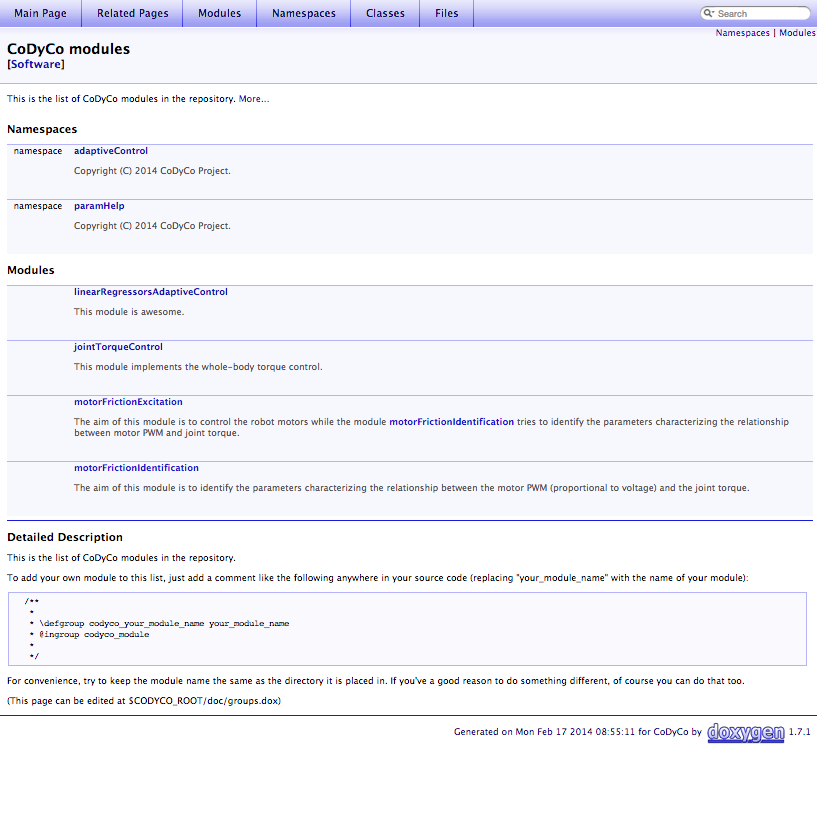
\includegraphics[width=0.45\textwidth]{images/docWeb.png} \\
\caption{The bottom left corner contains a screen-shot of the CoDyCo software documentation website \protect\url{http://wiki.icub.org/codyco/dox/html/index.html}. All the other images are screen-shots of the CoDyCo website \protect\url{www.codyco.eu}: main page (top-left), events-meetings (top-right) and results-videos (bottom-left).}
\end{figure}

\section{Technical details and design choices} \label{sec:tech}

The CoDyCo website is realized with Joomla,  free and open-source content management framework (CMS) for publishing web content. It is built on a model–view–controller web application framework that can be used independently of the CMS. The website can be either edited from the front end \url{www.codyco.eu} or from the back-end \url{http://codyco.eu/administrator}. Front-end editing is partial, restricted to certain web-pages and accessible only to registered users. Back-end editing is global and restricted only to administrators. 

%%\bibliographystyle{alpha}
%%\bibliography{main-bib}

\end{document}

%%% Local Variables:
%%% mode: latex
%%% TeX-master: t
%%% save-place: t
%%% End:
